\documentclass[nohyper,justified]{tufte-handout}
%\documentclass{article}
%\usepackage[absolute,showboxes]{textpos}
\usepackage[absolute]{textpos}
\usepackage{sidecap}
%\usepackage{color}
%\usepackage[usenames,dvipsnames,svgnames,table]{xcolor}
\usepackage{Sweave}
\begin{document}
\Sconcordance{concordance:timelyPF_Report1.tex:timelyPF_Report1.Rnw:%
1 7 1 1 0 14 1 1 52 6 1 1 4 1 2 7 1 1 4 12 0 1 2 7 1 1 3 19 0 1 2 7 1 1 %
4 18 0 1 2 6 1}

%\SweaveOpts{prefix.string=graphics/plot, eps = FALSE, pdf = TRUE}
 
\begin{wide}
\section{\Huge Performance Summary with Sweave and R}
{\Large Here is a little experiment with R and Sweave to produce a performance report.  I have done some samples in the past, but I wanted to iterate through a couple more, especially to evaluate other options for what has been started in the PApages package.  Of course, this text could be easily replaced with some commentary from a manager about opportunities, thoughts, or current allocation.  A dashboard set of charts also might be very helpful here.}
 
\hrulefill
 
\end{wide}
 
 
 
 
 
\begin{textblock*}{150mm}(5mm,70mm)
\begin{figure}
%to really fill the page, this works nicely
%\begin{minipage}[t]{1.2\linewidth}
%\begin{minipage}[t]{0.5\linewidth}
\vspace{0pt}
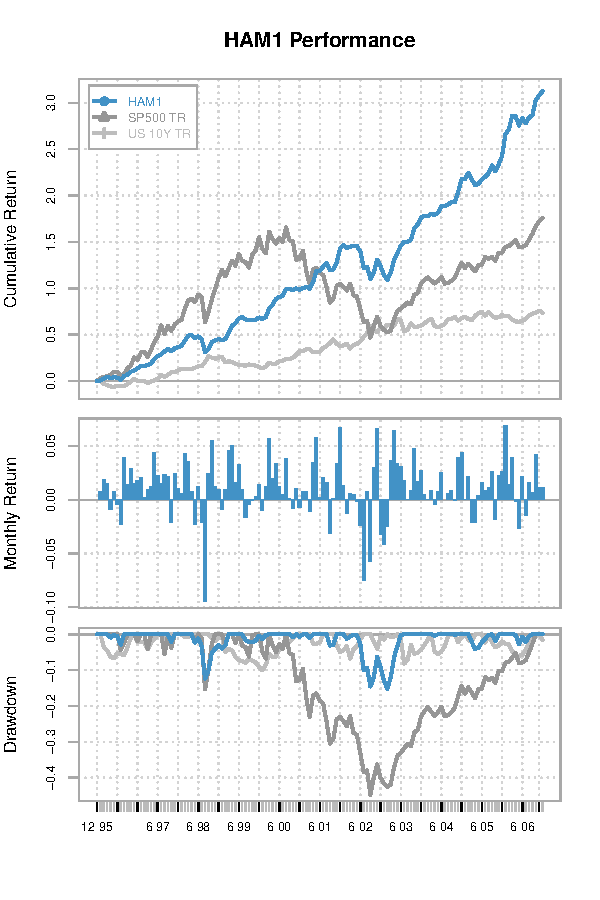
\includegraphics{timelyPF_Report1-002}
\end{figure}
\end{textblock*}
 
\begin{textblock*}{85mm}(120mm,103mm)
Cumulative returns offer one of the best methods to evaluate the ability of a manager to achieve long term returns.  Ultimately, the cumulative return is often one of the primary objectives of our clients.
\newline
\begin{figure}
\vspace{0pt}
% latex table generated in R 2.15.2 by xtable 1.7-1 package
% Mon Apr 29 14:21:04 2013
\scalebox{0.8}{
\begin{tabular}{rlll}
  \hline
 & HAM1 & SP500 TR & US 10Y TR \\ 
  \hline
1y & 1.60\% & 1.24\% & 0.12\% \\ 
  3y & 1.14\% & 0.85\% & 0.24\% \\ 
  5y & 0.92\% & 0.57\% & 0.41\% \\ 
  Since Inception  12 1995 & 1.10\% & 0.86\% & 0.44\% \\ 
   \hline
\end{tabular}
}\end{figure}
\end{textblock*}
 
\begin{textblock*}{85mm}(120mm,161mm)
However, cumulative returns must also be evaluated with reference to the risks incurred to generate those returns.  Below are multiple risk measures.  We are most concerned with limiting drawdowns shown in the bottom left chart.
\newline
\begin{figure}
\vspace{0pt}
% latex table generated in R 2.15.2 by xtable 1.7-1 package
% Mon Apr 29 14:21:04 2013
\scalebox{0.7}{
\begin{tabular}{rrrr}
  \hline
 & HAM1 & SP500 TR & US 10Y TR \\ 
  \hline
Semi Deviation & 0.02 & 0.03 & 0.01 \\ 
  Gain Deviation & 0.02 & 0.02 & 0.01 \\ 
  Loss Deviation & 0.02 & 0.03 & 0.01 \\ 
  Downside Deviation (MAR=10\%) & 0.02 & 0.03 & 0.02 \\ 
  Downside Deviation (Rf=0\%) & 0.01 & 0.03 & 0.01 \\ 
  Downside Deviation (0\%) & 0.01 & 0.03 & 0.01 \\ 
  Maximum Drawdown & 0.15 & 0.45 & 0.10 \\ 
  Historical VaR (95\%) & -0.03 & -0.07 & -0.03 \\ 
  Historical ES (95\%) & -0.05 & -0.09 & -0.04 \\ 
  Modified VaR (95\%) & -0.03 & -0.07 & -0.03 \\ 
  Modified ES (95\%) & -0.06 & -0.09 & -0.04 \\ 
   \hline
\end{tabular}
}\end{figure}
\end{textblock*}

\newpage
\section{Returns}
Unfortunately, the Return section is generally the focus of the sales pitch and also is often the biggest concern for the prospect.  Although it easiest to sell on return in the short-term, long-term success requires much more focus on the graphs presented in the Overview and Risk sections.
\begin{table}[htb]
\centering
% latex table generated in R 2.15.2 by xtable 1.7-1 package
% Mon Apr 29 14:21:04 2013
\begin{tabular}{rrrrrrrrrrrrr}
  \hline
 & 1 & 2 & 3 & 4 & 5 & 6 & 7 & 8 & 9 & 10 & 11 & 12 \\ 
  \hline
1995 &  &  &  &  &  &  &  &  &  &  &  & 0.00 \\ 
  1996 & 0.70 & 1.90 & 1.60 & -0.90 & 0.80 & -0.40 & -2.30 & 4.00 & 1.50 & 2.90 & 1.60 & 1.80 \\ 
  1997 & 2.10 & 0.20 & 0.90 & 1.30 & 4.40 & 2.30 & 1.50 & 2.40 & 2.20 & -2.10 & 2.50 & 1.10 \\ 
  1998 & 0.60 & 4.30 & 3.60 & 0.80 & -2.30 & 1.20 & -2.10 & -9.40 & 2.50 & 5.60 & 1.30 & 1.00 \\ 
  1999 & -0.90 & 0.90 & 4.60 & 5.10 & 1.60 & 3.30 & 1.00 & -1.70 & -0.40 & -0.10 & 0.40 & 1.50 \\ 
  2000 & -1.00 & 1.20 & 5.80 & 2.00 & 3.40 & 1.20 & 0.50 & 3.90 & 0.10 & -0.80 & 1.00 & -0.70 \\ 
  2001 & 0.80 & 0.80 & -1.10 & 3.50 & 5.80 & 0.20 & 2.10 & 1.60 & -3.10 & 0.10 & 3.40 & 6.80 \\ 
  2002 & 1.40 & -1.20 & 0.60 & 0.50 & -0.20 & -2.40 & -7.50 & 0.80 & -5.80 & 3.00 & 6.60 & -3.20 \\ 
  2003 & -4.10 & -2.50 & 3.60 & 6.50 & 3.40 & 3.10 & 1.80 & 0.00 & 0.90 & 4.80 & 1.70 & 2.80 \\ 
  2004 & 0.50 & -0.00 & 0.90 & -0.40 & 0.80 & 2.60 & 0.00 & 0.50 & 0.90 & -0.10 & 3.90 & 4.40 \\ 
  2005 & 0.00 & 2.10 & -2.10 & -2.10 & 0.40 & 1.60 & 0.90 & 1.10 & 2.60 & -1.90 & 2.30 & 2.60 \\ 
  2006 & 6.90 & 1.50 & 4.00 & -0.10 & -2.70 & 2.20 & -1.40 & 1.60 & 0.70 & 4.30 & 1.20 & 1.10 \\ 
   \hline
\end{tabular}%\caption{Unbelieveable returns with only one negative year.  SEC loves language like this.
%\label{fig:returns}}
\end{table}
\newpage
\section{Risk}

\end{document}
